\documentclass{article}

\usepackage{graphicx}
\usepackage{tikz}
\usepackage{tikzsymbols}
\usetikzlibrary{calc,patterns,shapes.geometric}
\pagestyle{empty}
\usepackage[margin=0pt]{geometry}
\geometry{papersize={14in,12in}}

\def\centerarc[#1](#2)(#3:#4:#5){\draw[#1] ($(#2)+({#5*cos(#3)},{#5*sin(#3)})$) arc (#3:#4:#5);}

\begin{document}
	\begin{figure}
		\centering
		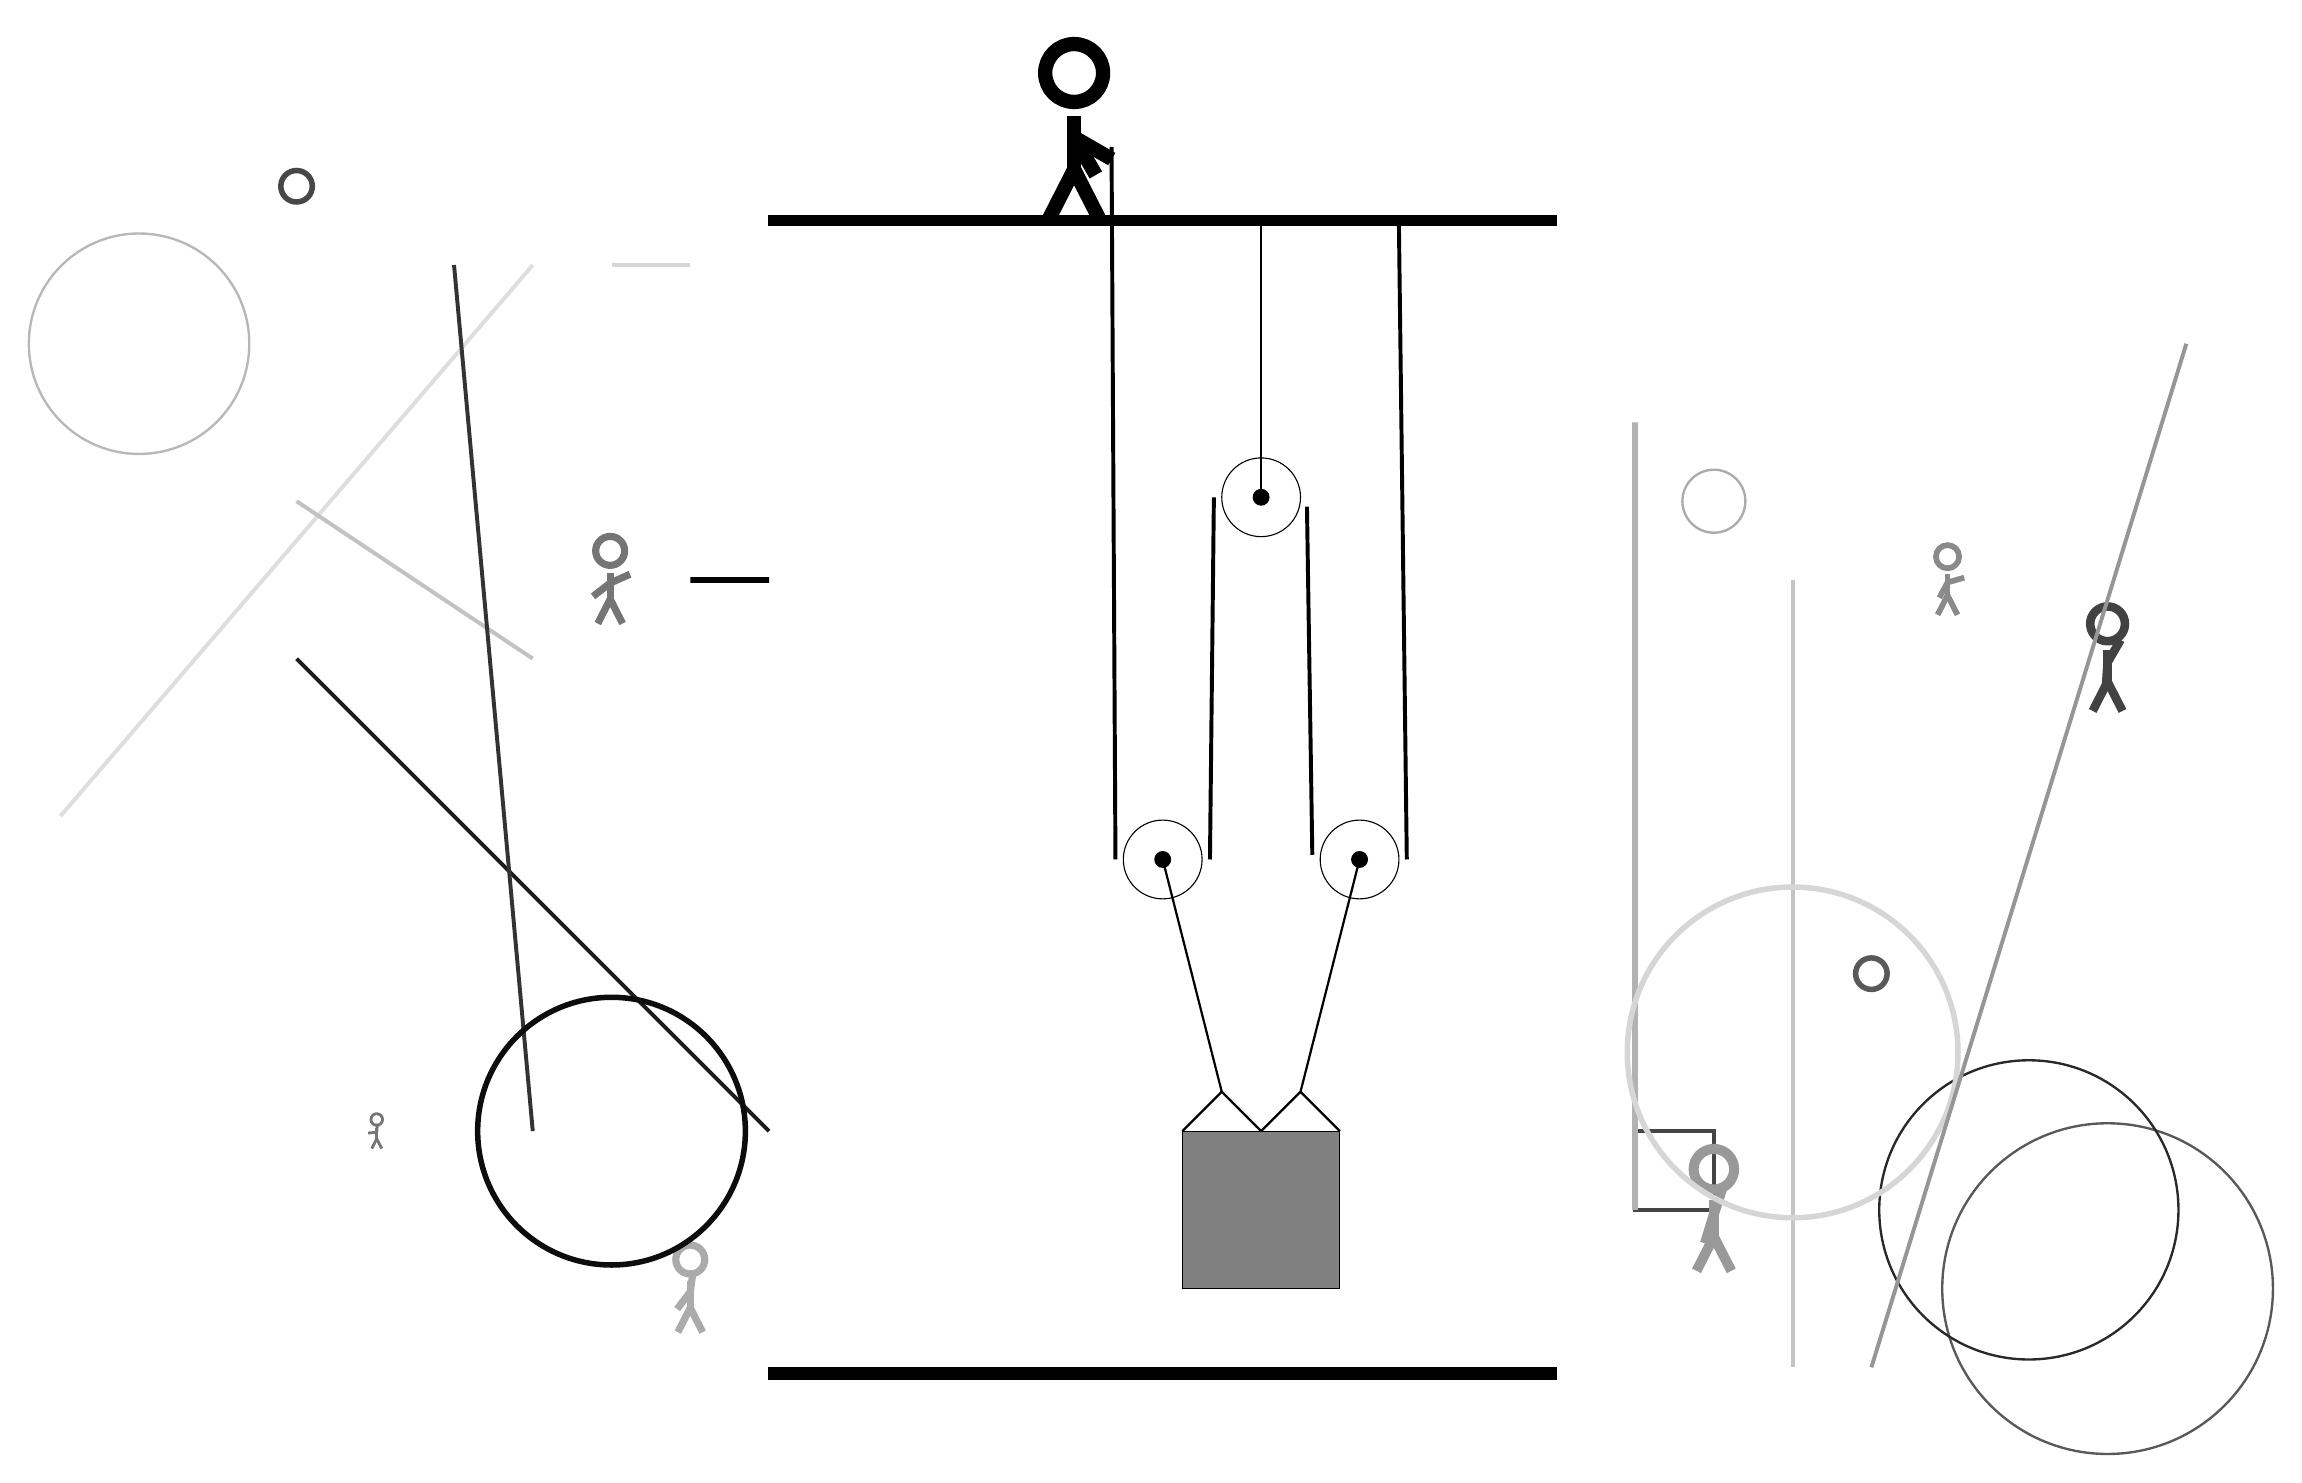
\begin{tikzpicture}
			%%%%% START %%%%%
			
			\draw[fill=black] (-4, 11.5) rectangle (6, 11.625);
			
			\draw (1, 3.45) circle (0.5);
			\draw[fill=black] (1, 3.45) circle (0.1);
			
			\draw (2.25, 8.05) circle (0.5);
			\draw[fill=black] (2.25, 8.05) circle (0.1);
			\draw[thick] (2.25, 8.05) -- (2.25, 11.5);
			
			\draw (3.5, 3.45) circle (0.5);
			\draw[fill=black] (3.5, 3.45) circle (0.1);
			
			\draw[thick] (3.5, 3.45) -- (2.75, 0.5);
			\draw[thick] (1, 3.45) -- (1.75, 0.5);
			\draw[thick]  (1.25, 0) -- (1.75, 0.5) -- (2.25, 0);
			\draw[thick]  (2.25, 0) -- (2.75, 0.5) -- (3.25, 0);
			\draw[fill=black!50] (1.25, 0) rectangle (3.25, -2);
			
			\draw[line width=0.5mm, color=black!89](-4, 0) -- (-10, 6);
			
			\draw [line width=0.7mm, color=black!65](10, 2) circle (0.2);
			\node[line width=0.4mm, color=black!74] at (13, 6) {\Strichmaxerl[6][86][60]};
			\draw[line width=0.5mm, color=black!13](-7, 11) -- (-13, 4);
			
			\draw[line width=0.5mm, color=black!23](9, 7) -- (9, -3);
			\draw [line width=0.3mm, color=black!28](-12, 10) circle (1.4);
			\draw [line width=0.3mm, color=black!65](13, -2) circle (2.1);
			
			\draw[line width=0.7mm, color=black!99] (-5, 7) rectangle (-4, 7);
			\draw [line width=0.7mm, color=black!72](-10, 12) circle (0.2);
			\draw[line width=0.5mm, color=black!73] (7, 0) rectangle (8, -1);
			
			\draw [line width=0.3mm, color=black!84](12, -1) circle (1.9);
			\draw[line width=0.5mm, color=black!24](-7, 6) -- (-10, 8);
			\node[line width=0.7mm, color=black!46] at (11, 7) {\Strichmaxerl[4][62][16]};
			
			\draw [line width=0.3mm, color=black!33](8, 8) circle (0.4);
			\node[line width=0.3mm, color=black!33] at (-5, -2) {\Strichmaxerl[5][53][82]};
			\draw[line width=0.5mm, color=black!80](-8, 11) -- (-7, 0);
			
			\node[line width=0.6mm, color=black!54] at (-6, 7) {\Strichmaxerl[5][38][24]};
			
			\draw [line width=0.7mm, color=black!95](-6, 0) circle (1.7);
			\draw[line width=0.5mm, color=black!16](-5, 11) -- (-6, 11);
			
			\draw[line width=0.7mm, color=black!30] (7, -1) rectangle (7, 9);
			\node[line width=0.7mm, color=black!40] at (8, -1) {\Strichmaxerl[7][73][72]};
			
			\draw [line width=0.7mm, color=black!16](9, 1) circle (2.1);
			\node[line width=0.4mm, color=black!54] at (-9, 0) {\Strichmaxerl[2][4][86]};
			\draw[line width=0.5mm, color=black!41](10, -3) -- (14, 10);
			
			\draw[line width=0.5mm] (0.35, 12.5) --  (0.4, 3.45);
			\centerarc[line width=0.5mm](1, 3.45)(180:360:0.6);
			\draw[line width=0.5mm] (1.6, 3.45) -- (1.65, 8.05);
			\centerarc[line width=0.5mm](2.25, 8.05)(-20:180:0.6);
			\draw[line width=0.5mm](2.832, 7.93) -- (2.9, 3.51);
			\centerarc[line width=0.5mm](3.5, 3.45)(160:360:0.6);
			\draw[line width=0.5mm](4.1, 3.45) -- (4.0, 11.5);
			
			\node at (-0.07, 12.7) {\Strichmaxerl[10][120][-30]};
			
			\draw[fill=black] (-4, -3) rectangle (6, -3.15);
			
			%%%%% END %%%%%
		\end{tikzpicture}
	\end{figure}	
\end{document}